% ****** Start of file aipsamp.tex ******
%
%   This file is part of the AIP files in the AIP distribution for REVTeX 4.
%   Version 4.1 of REVTeX, October 2009
%
%   Copyright (c) 2009 American Institute of Physics.
%
%   See the AIP README file for restrictions and more information.
%
% TeX'ing this file requires that you have AMS-LaTeX 2.0 installed
% as well as the rest of the prerequisites for REVTeX 4.1
%
% It also requires running BibTeX. The commands are as follows:
%
%  1)  latex  aipsamp
%  2)  bibtex aipsamp
%  3)  latex  aipsamp
%  4)  latex  aipsamp
%
% Use this file as a source of example code for your aip document.
% Use the file aiptemplate.tex as a template for your document.
\documentclass[%
 aip,
 jmp,%
 amsmath,amssymb,
%preprint,%
 reprint,%
%author-year,%
%author-numerical,%
]{revtex4-1}
\usepackage[utf8]{inputenc}
\usepackage[spanish]{babel}
\usepackage{graphicx}% Include figure files
\usepackage{dcolumn}% Align table columns on decimal point
\usepackage{bm}% bold math
%\usepackage[mathlines]{lineno}% Enable numbering of text and display math
%\linenumbers\relax % Commence numbering lines

\begin{document}

\preprint{AIP/123-QED}

\title[Laboratorio de Sísmica y Sismología]{Laboratorio de Sísmica y Sismología - Informe 1}% Force line breaks with \\
\thanks{Primer informe del Laboratorio de Sísmica y Sismología}

\author{Daniel Felipe Forero Sánchez}
 \altaffiliation{Departamento de Geociencias/Departamento de Física, Universidad de Los Andes}%Lines break automatically or can be forced with \\
 \email{df.forero10@uniandes.edu.co}
 \affiliation{201415069}
%\author{B. Author}%
% \email{Second.Author@institution.edu.}
%\affiliation{ 
%Authors' institution and/or address%\\This line break forced with \textbackslash\textbackslash
%}%

%\author{C. Author}
% \homepage{http://www.Second.institution.edu/~Charlie.Author.%}
%\affiliation{%
%Second institution and/or address%\\This line break forced% with \\
%}%

\date{\today}% It is always \today, today,
             %  but any date may be explicitly specified

\begin{abstract}
El presente informe muestra en detalle el trabajo realizado para el primer informe del Laboratorio de Sísmica y Sismología \cite{taller} de la Universidad de Los Andes en el primer semestre de 2016. Consiste en la creación de trazas sísmicas sintéticas dados dos diferentes casos de reflexión: incidencia normal y oblicua. Se utiliza el Método convolucional de trazas sísmicas en MATLAB y Python para la manipulación de datos, Microsoft Excel para cálculos sencillos y Seisee para la visualización de los archivos SEGY.
%

\end{abstract}


\keywords{Ondícula, Convolución, Traza sísmica, Coeficiente de reflexión}%Use showkeys class option if keyword
                              %display desired
\maketitle


\section{Introducción}

El método de convolución de trazas sísmicas consiste en calcular, a partir de una columna estratigráfica de la cual se conocen la densidad y velocidad de las ondas P ($v_P$) y S ($v_S$) de cada unidad, calcular el tiempo ($t$) en el cual la onda P es registrada tras la reflexión en cada una de las superficies reflectivas dados unos parámetros iniciales como el ángulo de incidencia ($\theta$).\\
Se usó la siguiente columna estratigráfica:
\begin{figure}[h]
\centering
\caption{Columna estratigráfica modelada}

\label{fig:Columna}
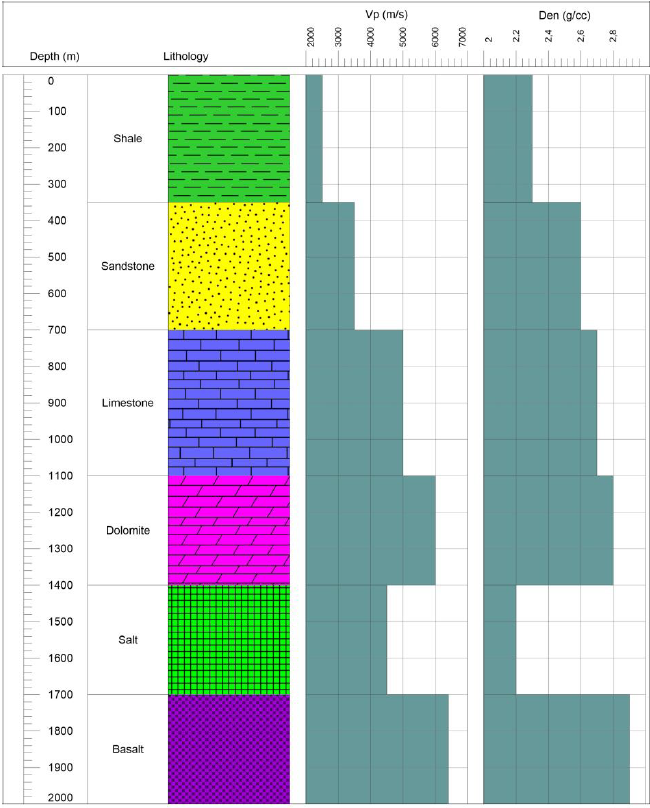
\includegraphics[width=0.7\linewidth]{Columna}
\end{figure}

En el cuadro \ref{tab:datos} se encuentran los datos necesarios obtenidos a partir de la columna estratigráfica.
\begin{table}[h]
	\centering
	\caption{Datos}
	\begin{tabular}{r|r|r|r|r|r}
		Hole ID & Techo $(m)$ & Base $(m)$ & Litologia & $v_P (m/s)$ & $\rho (g/cm^3)$ \\ \hline
		BH-1  & 0     & 350   & Lutita & 2500  & 2.3 \\
		BH-1  & 350   & 700   & Arenisca & 3500  & 2.6 \\
		BH-1  & 700   & 1100  & Caliza & 5000  & 2.7 \\
		BH-1  & 1100  & 1400  & Dolomita & 6000  & 2.8 \\
		BH-1  & 1400  & 1700  & Sal   & 4500  & 2.2 \\
		BH-1  & 1700  & 2000  & Basalto & 6400  & 2.9 \\
	\end{tabular}%
	\label{tab:datos}%
\end{table}%



\section{Procedimiento y Resultados}

En general, es necesario medir los tiempos en los cuales es registrada una onda sísmica enviada en $t=0$ después de ser reflejada en cada una de las superficies reflectivas (límites entre formaciones) e incluirlas en un arreglo de tiempos de una duración específica que representa el tiempo de muestreo; dicho arreglo tiene una cierta cantidad de elementos con una cierta separación, dicha separación permite definir la frecuencia del muestreo.

\subsection{Primer Experimento}
Se calcularon en Excel los tiempos ($t_{int}$) y tiempos acumulados ($t_{acc}$) en los cuales la señal reflejada en cada interfaz es recibida asi como las impedancias ($I$) y los coeficientes de reflexión ($R$) según las ecuaciones \ref{eqn:tint} a \ref{eqn:R1}, donde la ecuación \ref{eqn:tacc} describe la suma de los tiempos de viaje de todas las capas desde la superficial (lutita) hasta la capa de interés (capa).
\begin{eqnarray}
t_{int}=2\frac{espesor_{capa}}{v_{P, capa}}\\
\label{eqn:tint}
t_{acc, capa}=\Sigma_{i=lutita}^{capa}t_{int, i}\\
\label{eqn:tacc}
I=\rho v_P\\
\label{eqn:i1}
R=\frac{I_2-I_1}{I_2+I_1}
\label{eqn:R1}
\end{eqnarray}
Los datos obtenidos se muestran en la figura \ref{tab:tiemposExp1}.
% Table generated by Excel2LaTeX from sheet 'Hoja1'
\begin{table}[h]
	\centering
	\caption{Datos calculados para el experimento 1}
	\begin{tabular}{r|r|r|r}
		$t_{int}(ms)$ & $t_{acc}(ms)$ & $I (gm/cm^3s)$ & $R$ \\\hline
		280   & 280   & 5750  & 0.23 \\
		200   & 480.0 & 9100  & 0.19 \\
		160   & 640.0 & 13500 & 0.11 \\
		100   & 740.0 & 16800 & -0.26 \\
		133.3 & 873.3 & 9900  & 0.30 \\
		93.75 & 967.1 & 18560 & 0.00 \\
	\end{tabular}%
	\label{tab:tiemposExp1}%
\end{table}%

Con ayuda del software MATLAB se crea un vector de tiempo (tiempo de muestreo) de mil elementos (muestra de un segundo de duración e intervalo de muestreo de un segundo) en el cual se migran los ponen en los elementos $t_acc$ los valores $R$ de manera que se obtiene un vector de coeficientes de reflexión migrados en tiempo como se muestra en la figura.
\begin{figure}[h]
\centering
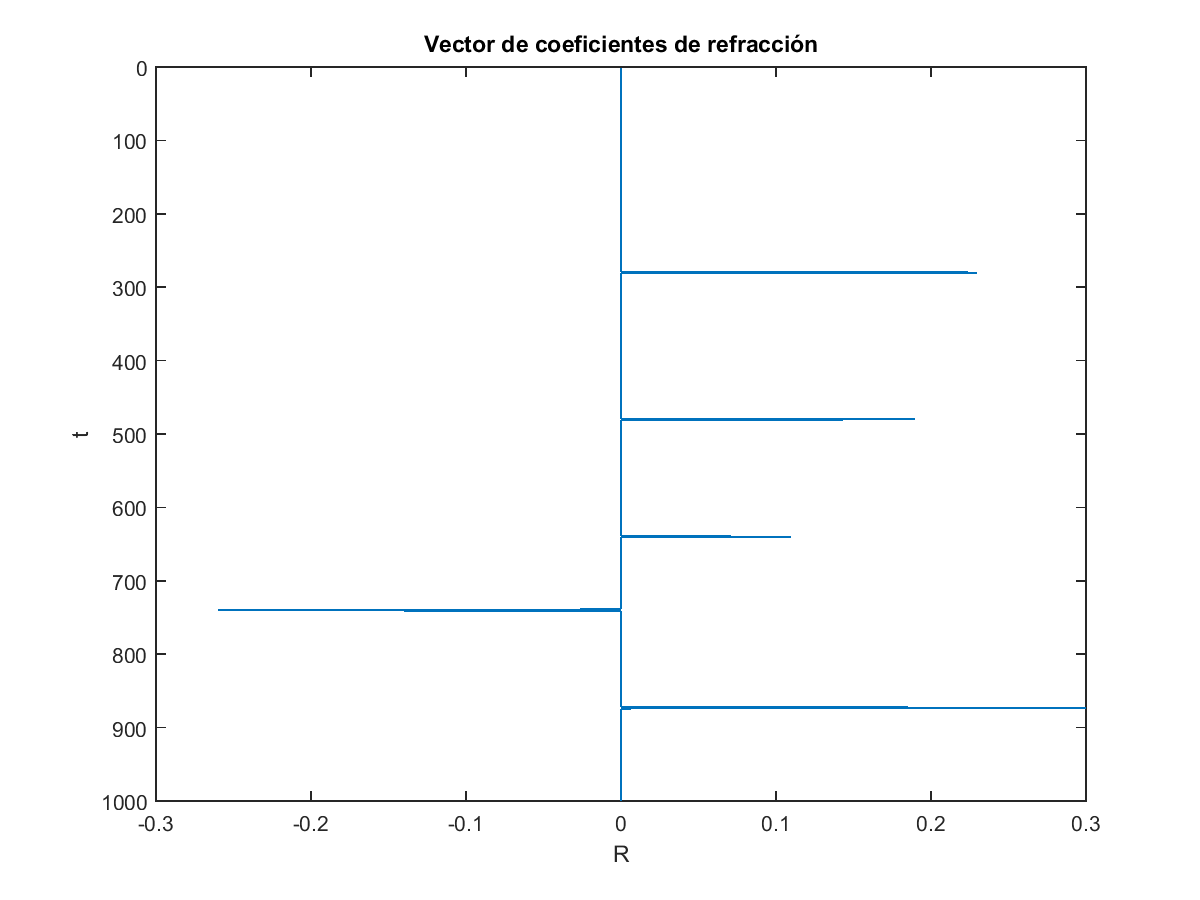
\includegraphics[width=1.\linewidth]{RC1}
\caption{}
\label{fig:RC1}
\end{figure}

Se crea la ondícula (de -2.5 a 2.5 con 20 elementos equivalentes a 20 milisegundos de duración) que se usará para la convolución, se usa la ondícula de Ricker mostrada


\begin{figure}[h]
\centering
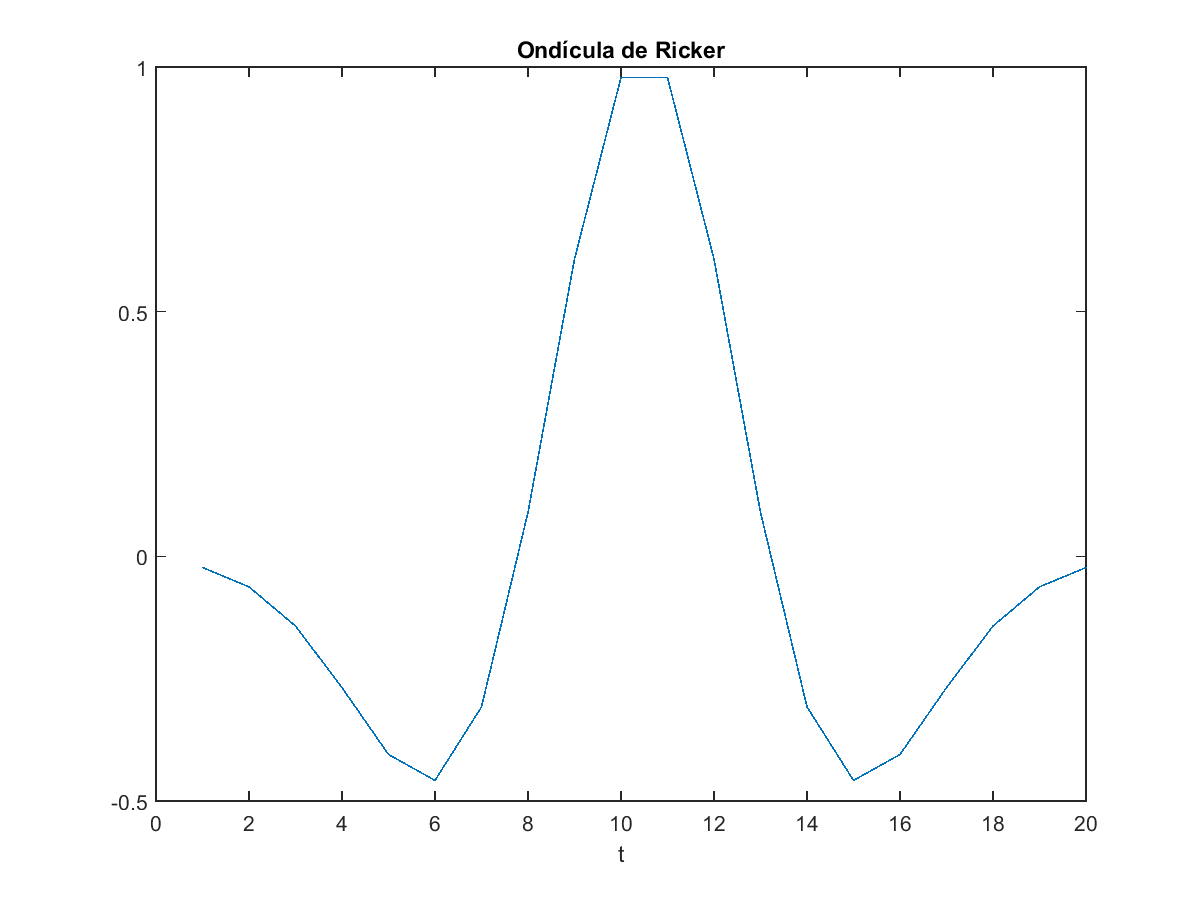
\includegraphics[width=1.\linewidth]{ondicula}
\caption{}
\label{fig:ondicula}
\end{figure}

Posteriormente se hace la convolución entre el vector de coeficientes de reflexión y la ondícula, obteniendo una traza sísmica con la siguiente forma.

\begin{figure}[h]
\centering
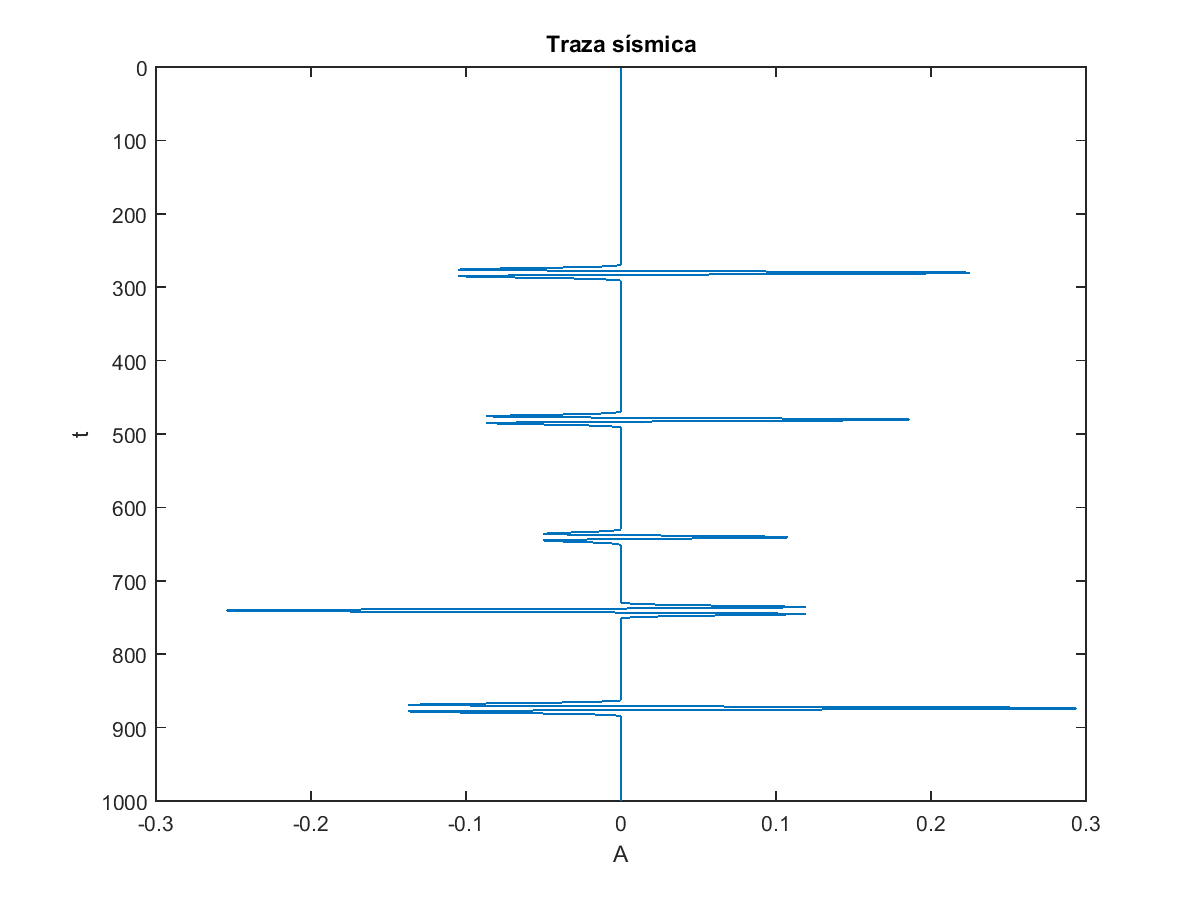
\includegraphics[width=1\linewidth]{TR1}
\caption{}
\label{fig:TR1}
\end{figure}

Finalmente a partir de esta traza se genera una matriz cuyos vectores columna son trazas sísmicas idénticas. Esta matriz se exporta a formato SEGY para ser visualizado en SeiSee (figura \ref{fig:seisee1}).

\begin{figure*}[!h]
\centering
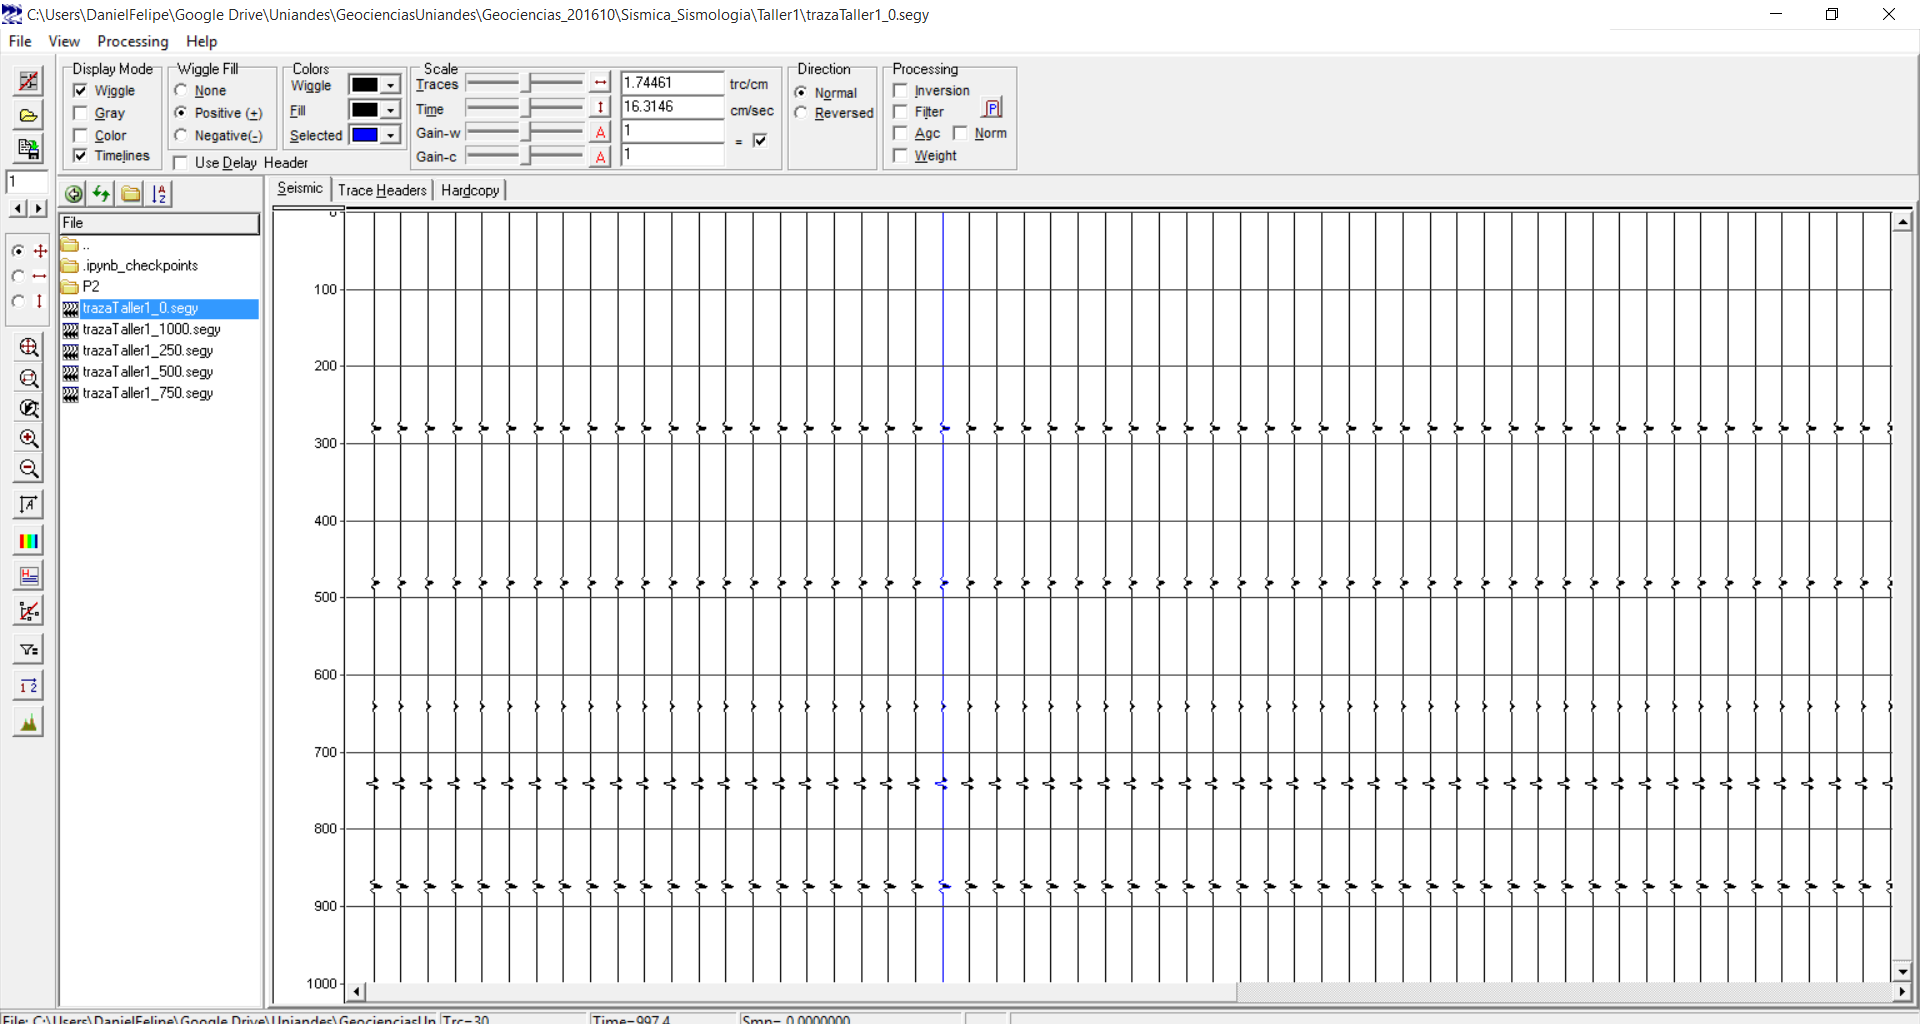
\includegraphics[width=1.\linewidth]{seisee1.png}
\caption{Visualización del archivo SEGY de cien trazas en SeiSee}
\label{fig:seisee1}
\end{figure*}

Se generan cuatro archivos más idénticos al mostrado en la figura \ref{fig:seisee1} de manera que se pueda editar el \textit{header} de cada archivo de forma que cada archivo represente las mediciones de una línea de sensores colocada 250m al este de la línea inicial. Para que cada traza del archivo muestre un arreglo de sensores se le dice al header del archivo, en el atributo 77 que la coordenada $y$ de cada traza es $10N$ donde $N$ es el número de la traza; para decirle que cada archivo representa una sola coordenada $x$ se escribe en el atibuto 73 que todas las trazas tienen un valor de 0, 250, 500, 750, o 1000, dependiendo del archivo. Posteriormente se cargan los archivos a OpendTect y se trazan las líneas que representan los reflectores en cada coordenada $x$, usando el software para interpolar y mostrar el reflector como una superficie 3D como se muestra en la figura \ref{fig:opend1}.

\begin{figure*}[!h]
	\centering
	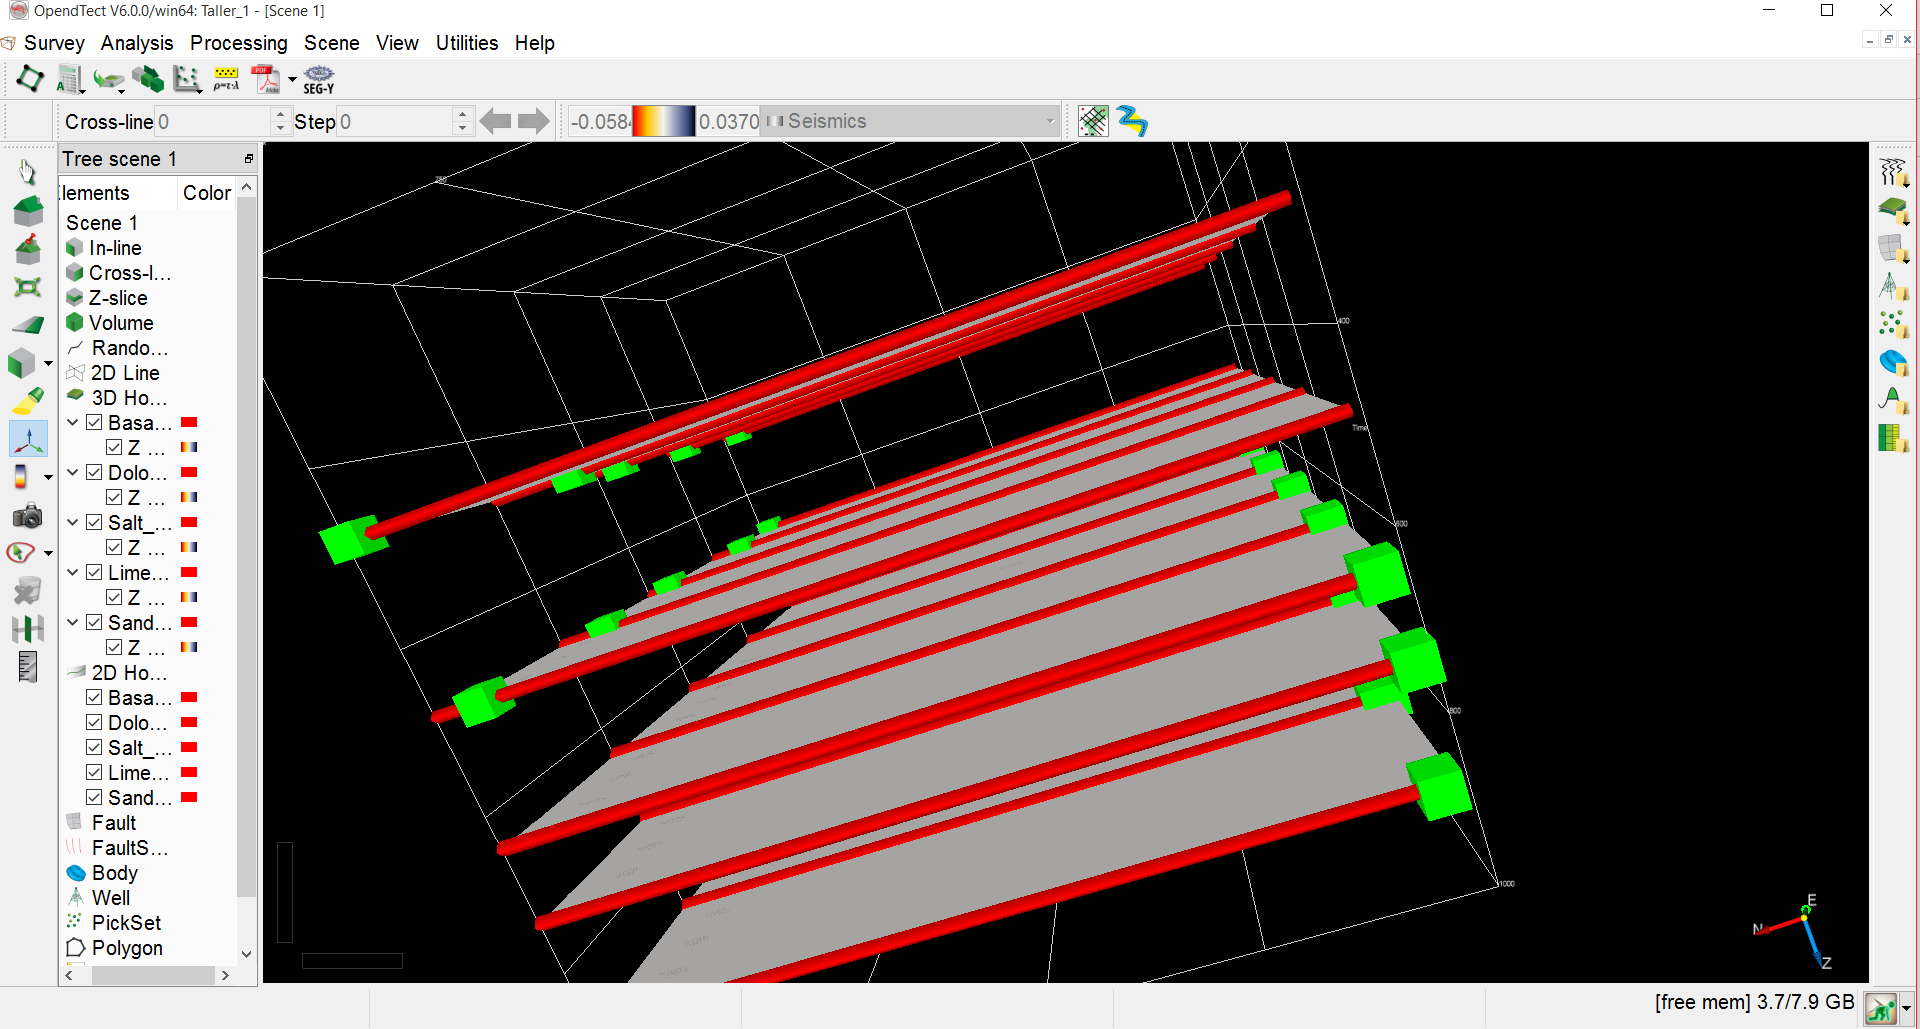
\includegraphics[width=1.\linewidth]{opend1.png}
	\caption{Visualización de los archivos de trazas como las superficies reflectivas propias de la estratificación supuesta para el experimento.}
	\label{fig:opend1}
\end{figure*}

\subsection{Segundo Experimento}

Cuando la incidencia de la onda sobre el reflector no es normal, el cálculo de los tiempos y coeficientes de reflexión no es tan trivial como en el experimento anterior, por lo que se definen las siguientes relaciones necesarias \ref{eqn:relacionesexp2}
\begin{subequations}
	\label{eqn:relacionesexp2}
\begin{equation}
t_{int}=\frac{2h}{v_{P}\cos(\theta_1)}\\
\label{eqn:tint2}
\end{equation}
\begin{equation}
\frac{\sin(\theta_1)}{v_{P1}}=\frac{\sin(\theta_2)}{v_{P2}}\\
\label{eqn:snell}
\end{equation}
\begin{equation}
\begin{aligned}
R_{PP}(\theta_1, \theta_2)\approx&\frac{1}{2}\ln\left(\frac{v_{P2}\rho_2\cos(\theta_1)}{v_{P1}\rho_1\cos(\theta_2)}\right)+\\
&\left(\frac{\sin(\theta_1)}{v_{P1}}\right)^2(v_{S1}^2-v_{S2}^2)\left[2+\frac{\ln(\rho_2/\rho_1)}{\ln(v_{S2}/v_{S1})}\right]
\end{aligned}
\label{eqn:approx}
\end{equation}
\end{subequations}
Donde $h$ es el espesor de la capa, $v_{Pi}$ es la velocidad de onda P en el medio $i$, $v_{Si}$ es la velocidad de onda S en el medio $i$. $R_{PP}(\theta_1, \theta_2)$ es la aproximación de Bortfeld para el coeficiente de reflexión de una onda P a onda P en la interfase entre dos medios 1 y 2. \\
Para el experimento necesitamos expresar $R_{PP}$ únicamente en función de $\theta_1$ por lo que se debe hacer uso de la relación \ref{eqn:snell} o Ley de Snell junto con la identidad $\cos^2(\theta)+\sin^2(\theta)=1$ para obtener la siguiente relación.
\begin{equation}
\cos(\theta_2)=\sqrt{1-\left(\frac{v_{P2}}{v_{P1}}\right)^2\sin^2(\theta_1)}
\label{eqn:identidad}
\end{equation}
Y reemplazando \ref{eqn:identidad} en \ref{eqn:approx}.
\begin{equation}
\begin{aligned}
R_{PP}(\theta_1)\approx&\frac{1}{2}\ln\left(\frac{v_{P2}\rho_2\cos(\theta_1)}{v_{P1}\rho_1\sqrt{1-\left(\frac{v_{P2}}{v_{P1}}\right)^2\sin^2(\theta_1)}}\right)+\\
&\left(\frac{\sin(\theta_1)}{v_{P1}}\right)^2(v_{S1}^2-v_{S2}^2)\left[2+\frac{\ln(\rho_2/\rho_1)}{\ln(v_{S2}/v_{S1})}\right]
\end{aligned}
\label{eqn:approxcorr}
\end{equation}

Se experimentará variando el ángulo de incidencia $\theta_1$ (de $0^{\circ}$ a $45^{\circ}$ en intervalos de $5^{\circ}$) sobre la primera superficie reflectiva, por lo que se calculan los tiempos de viaje de la onda ($t_{int}$) para cada uno de los $\theta_1$. Se calcula \ref{eqn:identidad} y posteriormente \ref{eqn:approxcorr}. Se genera un arreglo de coeficientes de reflexión de 400 elementos (400 ms de duración) y se desplaza cada coeficiente en el tiempo, obteniendo lo mostrado en la figura \ref{fig:rpps}.\\



\begin{figure*}[h]
\centering
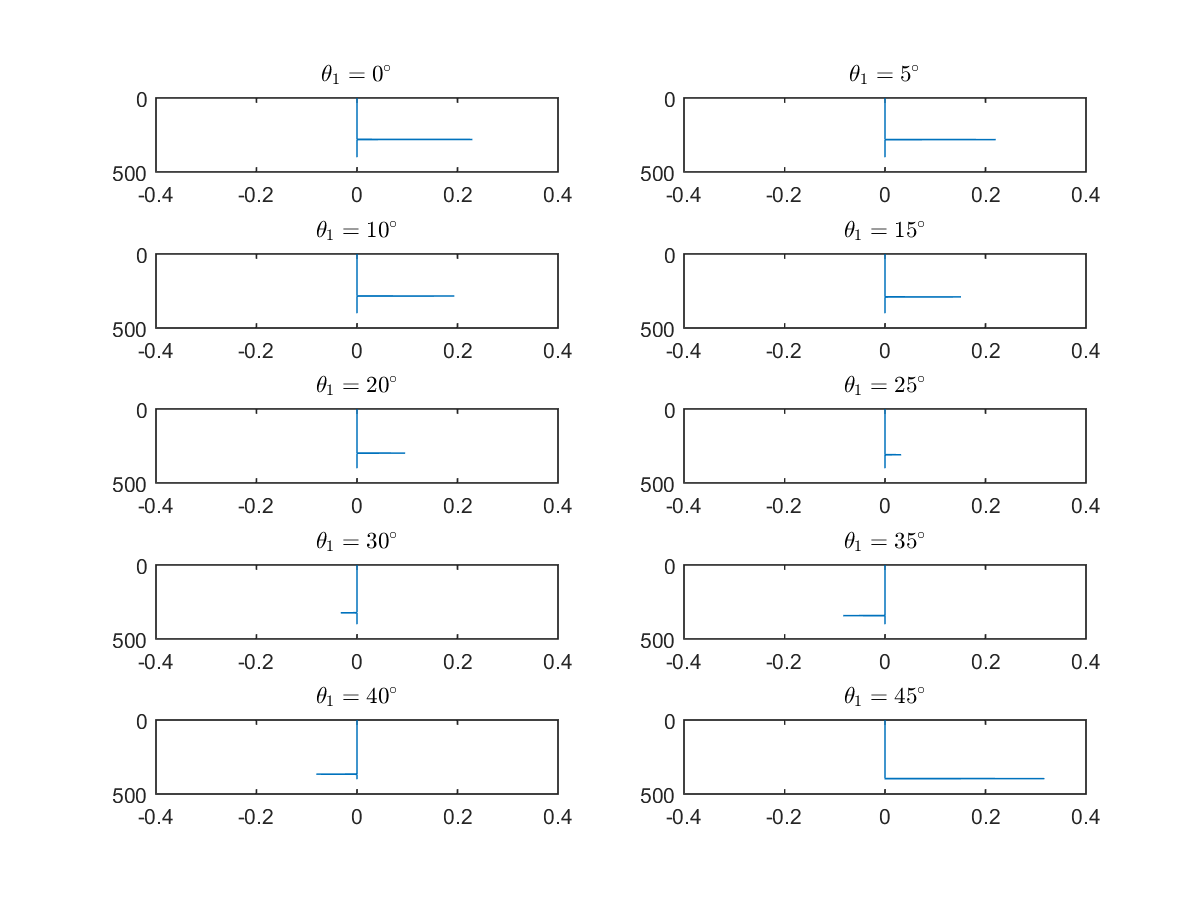
\includegraphics[width=1\linewidth]{rpps}
\caption{Arreglos de coeficientes de reflexión para cada $\theta_1$. Verticalmente:$t$. Horizontalmente:$R_{PP}$}
\label{fig:rpps}
\end{figure*}

Posteriormente se convuelven estos vectores con la ondícula del primer experimento para obtener lo mostrado en la figura \ref{fig:trazas2}.

\begin{figure*}[h]
	\centering
	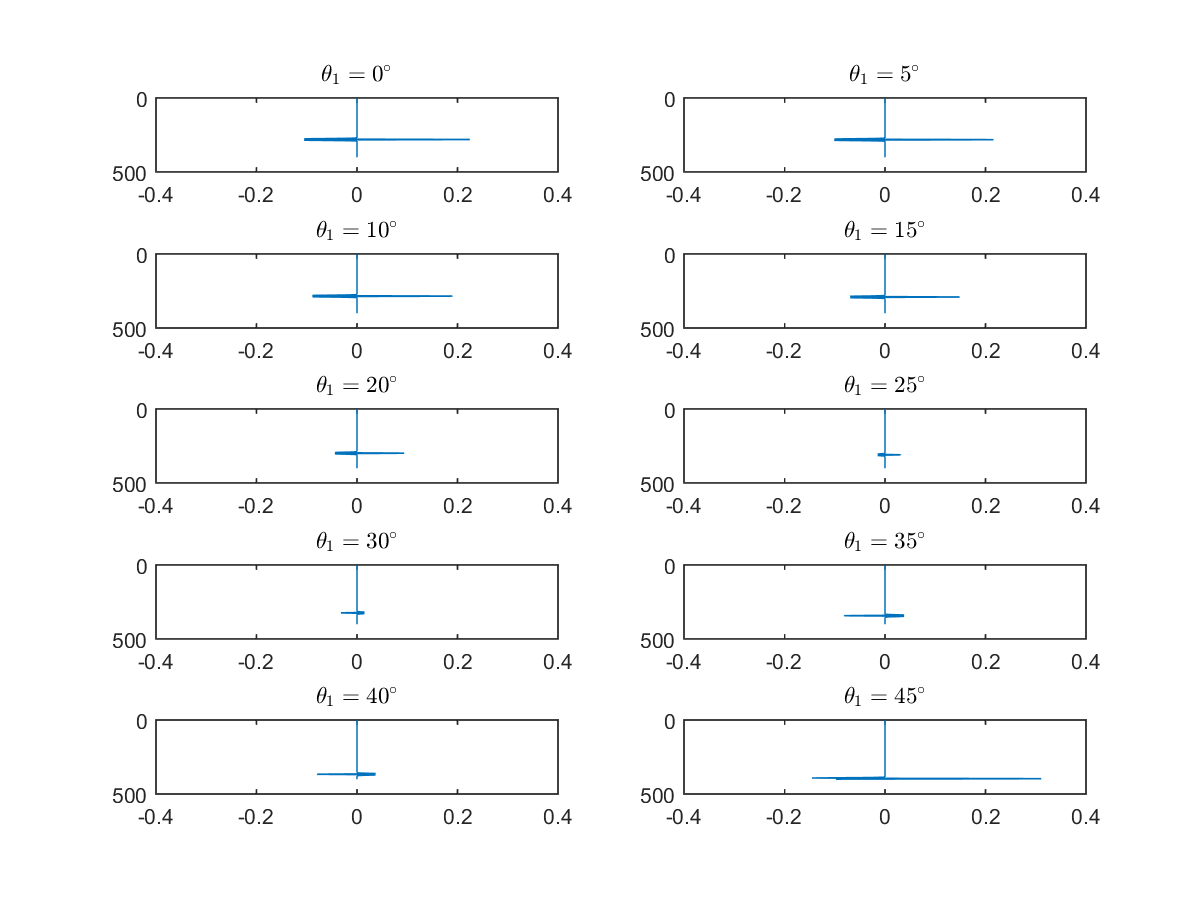
\includegraphics[width=1\linewidth]{trazas2}
	\caption{Trazas sísmicas obtenidas para cada $\theta_1$. Verticalmente:$t$.}
	\label{fig:trazas2}
\end{figure*}

Se construye una matriz cuyos vecotres columna sean las trazas recién obtenidas, y se exportan a un archivo SEGY que se abre en SeiSee (fig \ref{fig:exp2}).

\begin{figure*}[h]
\centering
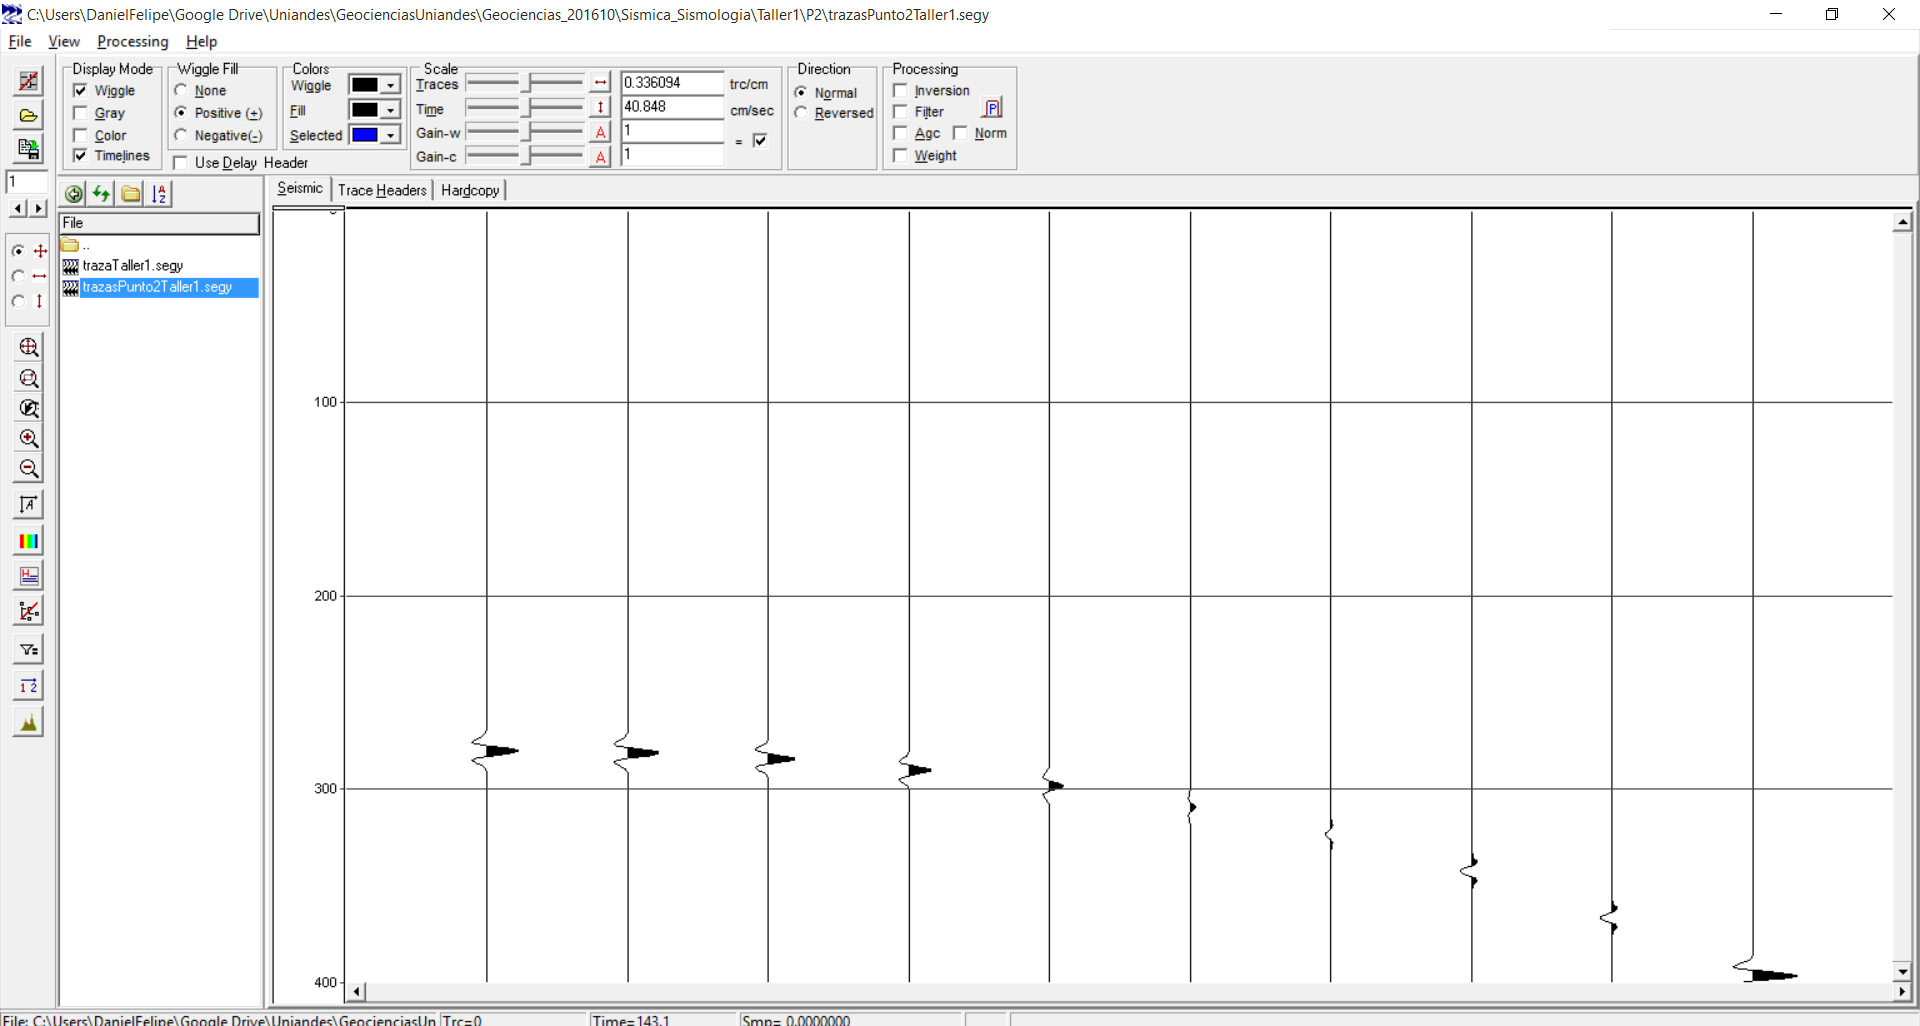
\includegraphics[width=1\linewidth]{exp2}
\caption{Visualización en SeiSee del segundo experimento, se ve la hipérbola esperada.}
\label{fig:exp2}
\end{figure*}

\section{Conclusiones}
\begin{enumerate}
	\item En el primer experimento se exploró la incidencia normal a una secuencia estratigráfica, que permitió modelar exitosamente una sección sísmica en 3D.
	\item Se implementó exitosamente el uso de software especializado como SeiSee y OpendTect.
	\item Se logró conocer más a fondo la estructura de los archivos SEGY de forma que se sepa manipular el encabezado para crear modelos de sísmica 3D.
	\item Se experimentó con un \textit{common shot gather}, comprendiendo las características de este \textit{gather} como lo es, por ejemplo la curva típica resultante (hipérbola).
\end{enumerate}

\bibliographystyle{unsrt}%Used BibTeX style is unsrt
\bibliography{export}

\end{document}
%
% ****** End of file aipsamp.tex ******
